
Performance measures to be optimized through learning are as diverse as the number of learning methods. In supervised binary classification, the generalization error defined as the misclassification rate on unseen or new data is considered to be the benchmark metric over which classifiers are optimized. 
In the sections below we discuss the relationship of each performance measure with the AMS metric and assess its relevance for the classification task at hand. 

Herein, we refer to the background class (N) as belonging to the majority class with a negative label of -1 and the signal class (P) as belonging to the minority class with a positive label of +1. 

\section{Importance Weights}

All the metrics described in the sections below are computed using importance weights $w_{i}$ rather than the count. Similar to the concept of a selection region $\mathcal{\hat{H}}$ introduced in eq. \ref{index_select} (section \ref{math}, chapter \ref{formal}) it is useful to introduce the notion of a rejection region that contains all events that fall outside of the selection region. It can be defined as, 

\begin{equation}
\mathcal{H}^{c} = \{\mathbf{x} : h(\mathbf{x}) = b\} = \{\mathbf{x} : f(\mathbf{x}) < \theta_{k}\}
\label{rejection}
\end{equation}

The index set of points that belong to the rejection region is given by, 

\begin{equation}
\mathcal{\hat{H}}^{c} = \{i : \mathbf{x}_{i} \in \mathcal{H}^{c}\} = \{i : h(\mathbf{x}) = b\} 
\end{equation}

Further, $\mathcal{H} \cap \mathcal{H}^{c} = \emptyset$ and $|\mathcal{H} \cup \mathcal{H}^{c}| = n$ where $n$ is the total  number of events in the dataset. Each event after classification is either in the selection region or the rejection region. 

Using the definitions of selection region and rejection region it is easy to enunciate the most commonly used terms in a binary classification context using importance weights:

\begin{table}[H]
\begin{center}
\begin{tabular}{c|c|c|c|c}
& & \multicolumn{2}{c}{Predicted Label}\\
\hline
& & -1 (b) & +1 (s) \\
\hline
\multirow{3}{*}{True Label} & -1 (b) & TN: $\sum_{i \in \mathcal{B} \cap \hat{\mathcal{H}^{c}}} w_{i}$  & FP($\hat{b}$): $\sum_{i \in \mathcal{B} \cap \hat{\mathcal{H}}} w_{i}$  & TN + FP = N\\ 
& +1 (s) & FN: $\sum_{i \in \mathcal{S} \cap \hat{\mathcal{H}^{c}}} w_{i}$ & TP($\hat{s}$): $\sum_{i \in \mathcal{S} \cap \hat{\mathcal{H}}} w_{i}$ & FN + TP = P\\ 
\hline 
\end{tabular}
\label{confusion_weights}
\caption{Classification terminology using weights}
\end{center}
\end{table}

The values falling in the second column (TP and FP) are directly used to determine the AMS metric $\dfrac{\hat{s}}{\sqrt{\hat{b}}}$.

\section{Accuracy: Training and Test error}

The training error is the misclassification rate of training samples and test error is the misclassification rate when a trained classifier is applied to unseen data points. Accuracy is (1 - misclassification rate) expressed as a $\%$.

As stated earlier, the error rates are a weak indicator of performance in the presence of imbalanced prior class distributions. A class with 99$\%$ samples of the majority class will achieve a 99$\%$ accuracy rate with a classifier that blindly assigns all samples to the majority class. 

In the Higgs dataset used for training and testing approximately 70$\%$ of the data points belong to the majority background class hence a classifier which achieves a 70$\%$ accuracy rate on test data is not a useful indicator of performance unless the measure is scrutinized further. 

\section{Recall and Precision}

The recall metric also called \textit{sensitivity} is computed as the fraction of the data points of the positive signal class correctly predicted as positive. Using the terminology described in table \ref{confusion_weights}, it is the fraction $\dfrac{\text{TP}}{\text{P}}$.  

The precision metric, is computed as the fraction of the predicted signals which are actually signals. It is the fraction, $\dfrac{\text{TP}}{\text{TP}+\text{FP}}$.

Since the AMS metric constitutes true positives (TP) and false positives (FP), the precision metric is a good indicator of AMS performance. 

\section{Balanced Classification error}

We have established that the overall classification accuracy in terms of count of events is a weak indicator of the strength of a classifier in the presence of unbalanced classes. A metric that effectively captures the fluctuations in the AMS must incorporate the importance weights $w_{i}$. One that is proposed by ATLAS physicists is the \textit{balanced classification error}. It is defined as, 

\begin{equation} 
R(f) = \sum_{i=1}^{n}w_{i}'\mathbb{I}\{y_{i}^{pred} \neq y_{i}^{true}\}. 
\label{bce}
\end{equation}

$\mathbb{I}$ is the indicator function. The weights $w_{i}'$ are normalized in both the signal and background classes to $N_{b}' = N_{s}' = 0.5$, that is, 

\begin{equation}
w_{i}' = w_{i}  \hspace{2mm} \times 
\begin{cases}
\dfrac{1}{2N_{s}} & \textrm{ if } i \in \mathcal{S} \\
\dfrac{1}{2N_{b}} & \textrm{ if } i \in \mathcal{B} 
\end{cases}
\label{neutralize}
\end{equation}

$N_s$ and $N_{b}$ denote the expected number of background and signal events as described in eq. \ref{unbiased}. 

It is important to neutralize the weights in this manner to compute the classification error in order to penalize misclassified signals as severely as misclassified background events. The original weights $w_{i}$ for signal events are on average 300 times smaller than those for background events. The balanced weights are generated only for the purposes of calculating the balanced classification error metric $R(f)$, the AMS is \textbf{always} computed on the unbalanced weights as in eq. \ref{weights}.

\begin{figure}
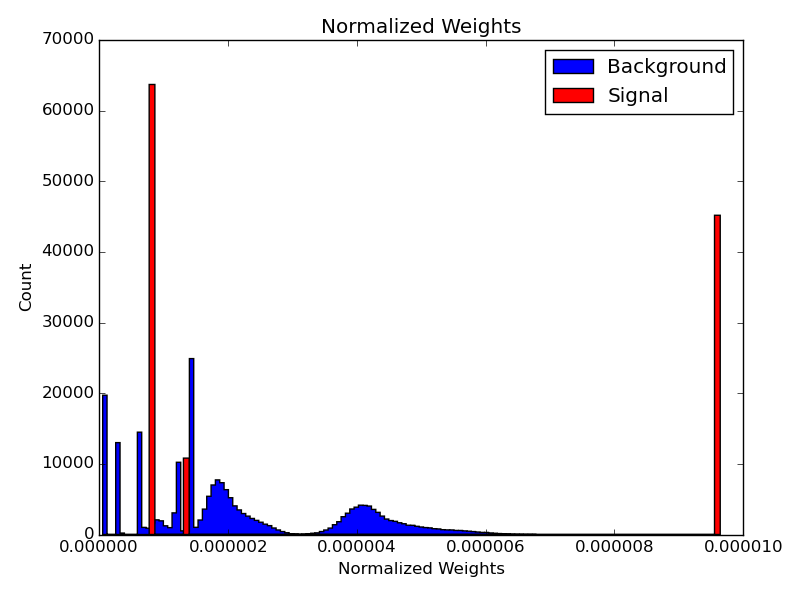
\includegraphics[width=\textwidth]{images/bweights.png}
\caption{Balanced weights for the signal and background classes.}
\label{bweights}
\end{figure}

Fig. \ref{bweights} shows the distribution of weights of the signal and background class after re-balancing them as per eq. \ref{neutralize}.

The magnitude of the balanced classification error of a classifier is a good indicator of AMS performance. Fine-tuning the parameters of a classifier to minimize this metric is an overwhelmingly popular approach. 

\section{Receiver Operator Characteristic (ROC)}

It is interesting to analyse the relationship between the simplified AMS metric $\hat{s}/\sqrt{\hat{b}}$ and the \textit{Receiver Operating Characteristic} (ROC) curve \footnote{The rather unusual name ROC emerged during World War II for the analysis of radar images. Radar operators had to decide whether a blip on the screen was an enemy target, friendly ship or just noise. Signal detection theory measures the ability of radar receiver operators to make these import distinctions. Their ability to do so was called \textit{Receiver Operating Characteristics}.}, they are closely related but not correlated. The ROC curve illustrates the performance of a binary classifier by depicting the true positive rate (TPR = TP/P), against the false positive rate (FPR = FP/N). A fixed threshold $\theta_{k}$ gives a single TPR and FPR (a single point on the curve), the curve is generated by computing the TPR and FPR for different values of $\theta_{k}$. Fig. \ref{roc} is an example of ROC curves for 3 different classifiers. 

\begin{figure}
\begin{center}
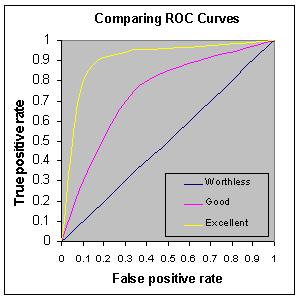
\includegraphics[scale=3]{images/Comparing_ROC.jpg}
\caption{ROC curves for classifiers with different levels of prediction accuracy. Adapted from \cite{roc}.}
\end{center}
\label{roc}
\end{figure}

The $45^\circ$ line denotes a random classifier, which at no threshold gives a higher TPR than FPR. A ROC curve that lies above the $45^\circ$ denotes a classifier with higher than random classification accuracy of positive samples for all values of the threshold and encloses a larger area under the curve. A perfect classifier has a TPR = 1 and FPR = 0 denoting perfect accuracy. The closer the ROC curve for a classifier is to the upper left corner of the graph (1,0) the better the classifier. The value on the $x$-axis, the FPR is also expressed as (1 - \textit{specificity}), where  specificity is the true negative rate (TN/N). Optimizing a classifier for the ROC curve pulls the curve towards the upper left corner of the graph to give higher true positive rates for each false positive rate.   

It seems as though then the threshold $\theta_{k}$ which corresponds to the upper left most point on the ROC curve should correspondingly maximize the AMS, however that is not the case and it is not immediately apparent as to why. 

I offer two explanations for this.

\begin{enumerate}

\item By ROC standards when choosing between two classifiers, the classifier that generates a higher ROC curve and encloses a greater area underneath it is the more optimal one, the area under the ROC curve is shortened as ROC$\_$AUC. The ROC$\_$AUC integrates across all possible choices of the threshold $\theta_{k}$. The threshold that corresponds to the upper left most point on the curve is chosen as the optimal threshold $\theta_{k}$. 
By AMS standards, we are concerned with the TPR and FPR values at a single optimal choice of threshold $\theta_{k}$. Effectively, this is a single point on the ROC curve. The shape or height of the ROC curve does not matter. We can achieve the same optimal AMS value on two very different ROC curves. 

\item Further, there is no guarantee that the AMS is maximized at the upper left most point of the ROC curve. The upper left most point on the ROC curve is the point which maximizes the ratio TPR/FPR. This ratio is the slope of the tangent to the ROC curve at a single point. The next section describes this ratio and contrasts it with the behaviour of the AMS.   

\end{enumerate}

In summary, optimizing for ROC is not equivalent to optimizing for AMS. 

\section{Likelihood Ratio}

The slope of the tangent line to the ROC curve at a fixed threshold $\theta_{k}$ is the ratio $\dfrac{\textrm{TPR}}{\textrm{FPR}}$. This is also called the positive likelihood ratio $(\textrm{LR}+)$, 

\begin{equation} 
\textrm{LR}+ = \frac{\textrm{TPR}}{\textrm{FPR}} = \frac{sensitivity}{(1 - specificity)} 
\end{equation}

It is easy to see that this ratio is maximised at the extreme upper-left hand corner of the ROC curve, this is the point that gives the best trade-off between  the true positive rate and false positive rate. It is a reasonable approach in classification to maximise the LR+ of a classifier in order to improve its overall classification accuracy.

Recall that the AMS metric $(\hat{s}/\sqrt{\hat{b}})$ is essentially the ratio of true positives to false positives in a selection region $\mathcal{H}$ specified by a cut-off threshold $\theta_{k}$. Maximizing the AMS is tantamount to maximizing the true positives and minimizing the false positives in the selection region. This seems very close to the idea of maximizing the positive likelihood ratio $(LR+)$. However, there are some fundamental differences.

\begin{enumerate}
\item The likelihood ratio uses true positive and false positive rates while the AMS uses unnormalized sums.

\begin{equation}
\textrm{ LR+: } \dfrac{\hat{s}/N_{s}}{\hat{b}/N_{b}} = \frac{\sum_{i \in \mathcal{S}\cap\hat{\mathcal{H}}} w_{i}/\sum_{i \in \mathcal{S}}w_{i}}{\sum_{i \in \mathcal{B}\cap\hat{\mathcal{H}} w_{i}}/\sum_{i \in \mathcal{B}}w_{i}}
\end{equation}

\begin{displaymath}
\textrm{ AMS: }\frac{\hat{s}}{\sqrt{\hat{b}}} = \frac{\sum_{i \in \mathcal{S}\cap\hat{\mathcal{H}}} w_{i}}{\sqrt{\sum_{i \in \mathcal{B}\cap\hat{\mathcal{H}}} w_{i}}}
\end{displaymath}

This distorts the correlation between the likelihood ratio and AMS metric. It is possible to achieve a higher AMS metric at a point on the ROC curve where the LR+ ratio is not maximized.

\item{The AMS ignores all samples that lie in the rejection region like false negatives (signals predicted to be background), however, LR+ is sensitive to it,
\begin{center}
TPR = TP/P = TP/(TP + FN)
\end{center}} 
The AMS using these metrics is simply, TP/$\sqrt{\textrm{FP}}$.

\end{enumerate}

\section{AMS (\texorpdfstring{$\sigma$}{s})}

\label{metrics}

A classifier is trained to minimize the balanced classification error as in eq. \ref{bce}. The AMS is then optimized with respect to a threshold $\theta_{k}$ in the classifier that generates a selection region $\mathcal{H} = \{\mathbf{x}: f(\mathbf{x}) > \theta_{k}\}$ with predicted signals. This is tantamount to classifying according to the rule,  $\sign\left(f\left(\mathbf{x}\right) - \theta_{k}\right)$. Prior experiments at ATLAS suggest that the AMS is maximized at a threshold $\theta_{k}$ yielding a selection region of the top $15\%$ of the events ranked by score. This implies selecting $\theta_{k}$ as the 85th percentile value of the score $f(\mathbf{x})$. Direct optimization of the AMS metric is infeasible as it is fully determined by the small number of events in the selection region $\mathcal{H}$, this makes it noisy and ill-conditioned since a small perturbation in the classifier can lead to a different composition of events in the selection region and a different value of the AMS. The suggested approach is a two step process. 

\begin{enumerate}
\item  Fine tune the classifier performance treating the balanced classification error as a loss function. 
\item Fine tune the choice of threshold $\theta_{k}$ for the classifier optimized in Step 1 through optimization of the AMS.   
\end{enumerate}

From a machine learning point of view the Higgs dataset represents two fundamental challenges described in the sections below.

\section{Class imbalance \texorpdfstring{\&}{} Class overlap}

Studies show that there are at least two main sources of difficulty in classification problems - one of them is class overlap and the other is class imbalance. Class imbalance refers to the under-representation of one or more class labels in the training and test data .i.e., a difference in class prior probabilities. Class overlap exacerbates the problem of class imbalance. In order to illustrate the conjecture consider the case of a single attribute problem with two classes. The probability distribution of the attribute values of the two classes are given by the gaussian distributions with the same variance but different means. In figure \ref{more} below the mean of the class represented by the dashed line (positive class) is one standard deviation away from the mean of the class represented by the solid line (negative class). The vertical lines denotes the optimal split. It is easy to see that the influence of changing prior probabilities of the positive class on the optimal split is much greater in the highly overlaid instances, in fig. \ref{more} than in fig. \ref{less} where the instances are well separated. In fig. \ref{less} where the mean of the positive class represented by the dashed line is four standard deviations away from the negative class, the optimal split derived by a simple classifier is inelastic to the changing priors \cite{overlap}.

\begin{figure}[H]
\centering
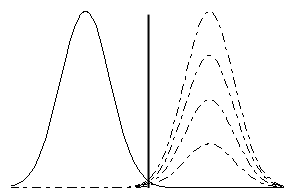
\includegraphics[scale=0.5]{images/loverlap}
\caption{Well separated classes}
\label{less}
\end{figure}

\begin{figure}[H]
\centering
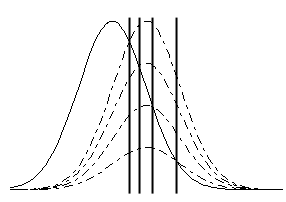
\includegraphics[scale=0.5]{images/hoverlap}
\caption{Overlaid classes}
\label{more}
\end{figure}

\section{Bias-Variance trade-off}

In machine learning parlance the bias-variance trade-off refers to the problem of balancing model accuracy and model generalization ability, it is usually impossible to improve both simultaneously. A highly accurate model that captures the regularities of the training data well is a low-bias model. A low-bias model comes at the cost of high model complexity which can lead to the problem of over-fitting. An over-fitted model is sensitive to small fluctuations in the training data set. Even a slight perturbation of the training data leads to a substantially different model structure. Hence, low bias usually occurs with high variance. 

On the flip side, a simple model which is more deterministic in its output is a high-bias low-variance model. It is too simple to capture the hidden relationships between the training data and output leading to high-bias (low accuracy) and under-fitting but has low variance. An under fitted model is stable to small perturbations in the training data. Hence, high bias usually occurs with low variance.

\begin{figure}[ht]
\begin{center}
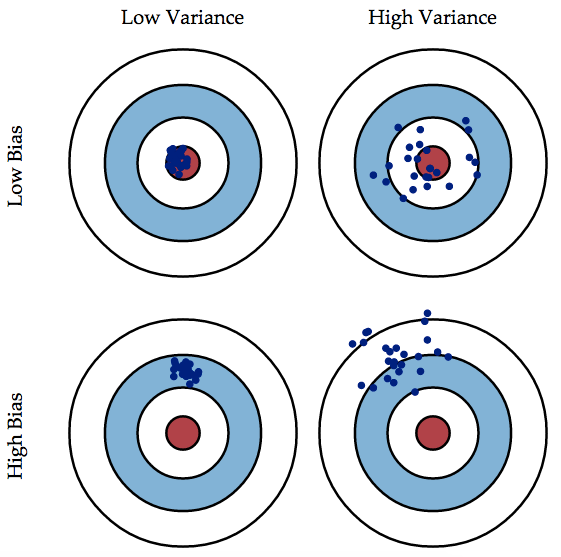
\includegraphics[scale=0.5]{images/biasvariance.png}
\caption[Bias-Variance Depiction]{This figure illustrates the different combinations of bias and variance. The red  center represents the target that the points need to fit to. The concentric circles represent different levels of diffusion. Low bias-low variance models present a theoretical standard - this is where models want to be. High-bias high variance models represent the attributes of an ill-defined model. Most models fall into the other two categories of being either low-bias high-variance or high-bias low-variance. Adapted from \cite{tradeoff}.}
\end{center}
\end{figure}

The error or misclassification rate on the training data is usually used to measure bias of a model and the variance of the output predictions of a model capture the variance of a model. The negative relationship between bias and variance of a model make it difficult to moderate both measures simultaneously. 

Robust models usually lie somewhere in the middle of the bias-variance spectrum with an acceptable amount of bias and variance. The goal of parameter optimization is usually to find this point on the bias-variance trade-off curve.

\begin{figure}[ht]
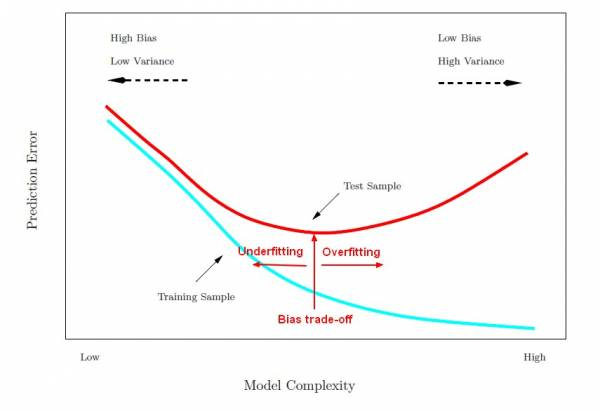
\includegraphics[width=\textwidth]{images/model_complexity_error_training_test.jpg}
\caption[Bias-Variance vs. Model Complexity]{The red curve depicts prediction/generalization error, the blue curve depicts training error. The diagram depicts that it is possible to achieve arbitrarily accurate models in fitting to a training dataset, such models usually define complex rules to capture the hidden relationships in training data. However, the effectiveness of such models on unseen data is poor as they are too over-fitted to the training set. There is a cross-over point where the error on test data starts to degrade. Good models position themselves at the point when this starts to happen. Adapted from \cite{complexity}.}
\label{complexity}
\end{figure}
